roughly 2-3 pages
\begin{itemize}
\item any details about experiments (dataset sizes, parameter selection, etc)
\item results
\item analysis (discussion of results/visualizations/findings/etc)
\end{itemize}

The experiments have been run on a dataset consisting of $9.728$ labeled documents. Different parameters may influence the accuracy of the classifier.These are $\alpha$, the Dirichlet parameter for $\theta$, $\beta$, the Dirichlet parameter for $\varphi$, the number of topics to be extracted from the dataset and the number of iterations for Gibbs sampling. 
For validation, k-fold cross-validation has been used with $k=4$, to ensure an unbiased test.

\subsection{Results}
Figure \ref{fig:topicdist} presents genre profiles for different genres. Each profile is created by summing topic counts for every document in the genre, and averaging these. These profiles are strongly dominated by one or two topics for certain genres, like \textit{Holiday}, \textit{Religious} and \textit{Reggae}, but more evenly distributed for others, like \textit{Electronic} or \textit{Pop/Rock}. This is not surprising, as \textit{Holiday} and \textit{Religious} are genres named after the themes of their songs, and not their musical structure. Moreover, \textit{Pop/Rock} contains music styles ranging from pop music to brutal death metal, resulting in a genre profile that covers a wide range of topics.

It can be seen that the extension of LDA puts out more sensible topics than regular LDA: for example, after 20 iterations, the top words of the top topic of the reggae genre are \verb|yeah|, \verb|get|, \verb|got|, \verb|right|, \verb|man|, \verb|like|, \verb|little|, \verb|time|, \verb|say| and \verb|hey| using regular LDA, and \verb|mi|, \verb|fight|, \verb|police|, \verb|gonna|, \verb|say|, \verb|jah|, \verb|whatcha|, \verb|dem|, \verb|ya|, \verb|yuh|, \verb|burnin| and \verb|ah| using the extension of LDA. \textbf{VERMOEDEN, KAN PAS NA TESTS ECHT GEZEGD WORDEN} This results in a more effective classifier: \textbf{INSERT RESULTS.}

\begin{figure}
        \centering
        \begin{subfigure}[b]{0.3\textwidth}
                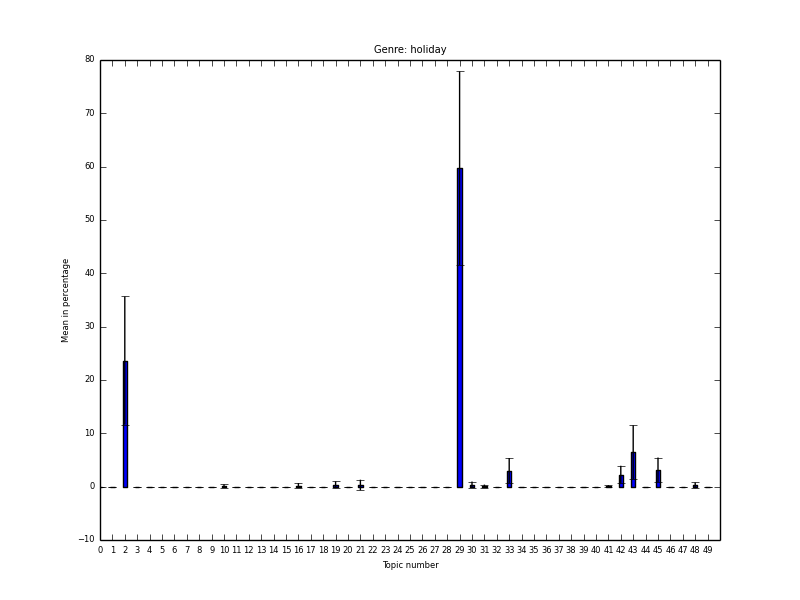
\includegraphics[width=\textwidth]{bar_charts/holiday.png}
                \caption{Genre Holiday}
                \label{fig:topicdist_holiday}
        \end{subfigure}%
        ~ %add desired spacing between images, e. g. ~, \quad, \qquad, \hfill etc.
          %(or a blank line to force the subfigure onto a new line)
        \begin{subfigure}[b]{0.3\textwidth}
                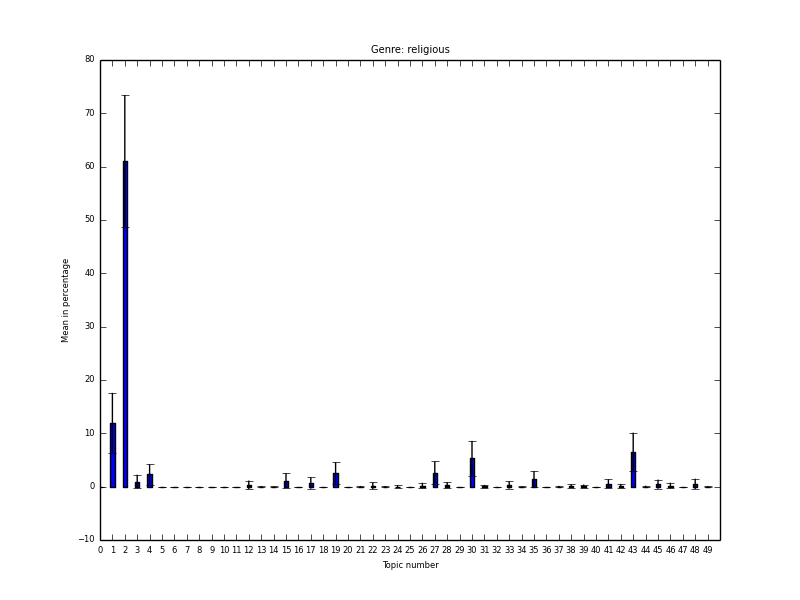
\includegraphics[width=\textwidth]{bar_charts/religious.png}
                \caption{Genre Religious}
                \label{fig:topicdist_religious}
        \end{subfigure}
        ~ %add desired spacing between images, e. g. ~, \quad, \qquad, \hfill etc.
          %(or a blank line to force the subfigure onto a new line)
        \begin{subfigure}[b]{0.3\textwidth}
                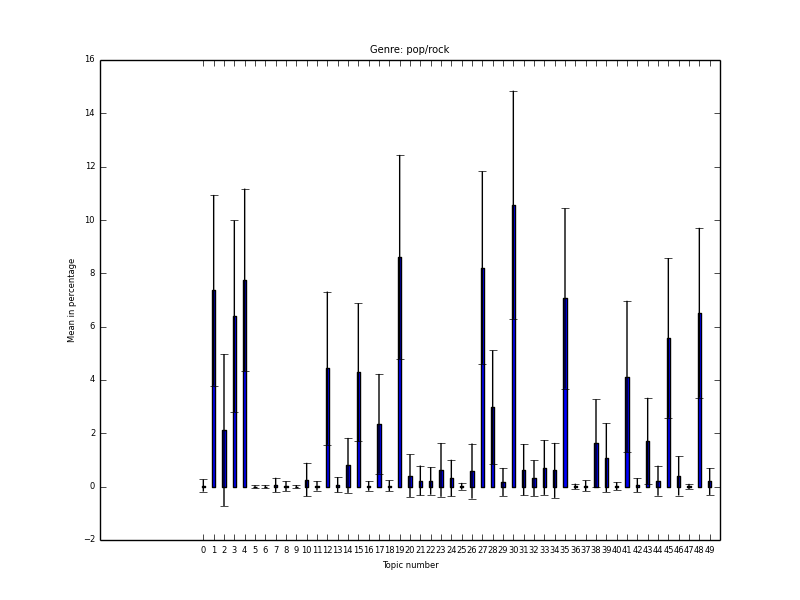
\includegraphics[width=\textwidth]{bar_charts/pop-rock.png}
                \caption{Genre Pop/Rock}
                \label{fig:topicdist_poprock}
        \end{subfigure}
        \begin{subfigure}[b]{0.3\textwidth}
                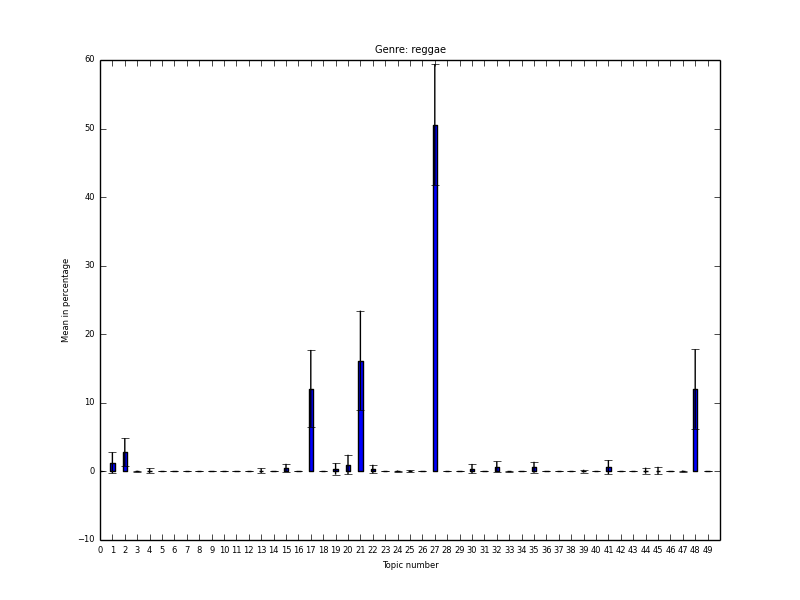
\includegraphics[width=\textwidth]{bar_charts/reggae.png}
                \caption{Genre Reggae}
                \label{fig:topicdist_reggae}
        \end{subfigure}%
        ~ %add desired spacing between images, e. g. ~, \quad, \qquad, \hfill etc.
          %(or a blank line to force the subfigure onto a new line)
        \begin{subfigure}[b]{0.3\textwidth}
                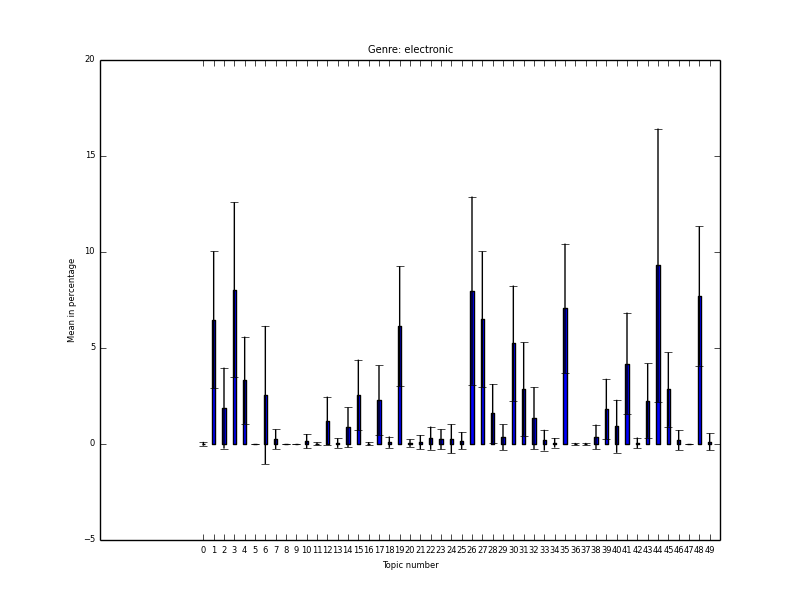
\includegraphics[width=\textwidth]{bar_charts/electronic.png}
                \caption{Genre Electronic}
                \label{fig:topicdist_electronic}
        \end{subfigure}
        ~ %add desired spacing between images, e. g. ~, \quad, \qquad, \hfill etc.
          %(or a blank line to force the subfigure onto a new line)
        \begin{subfigure}[b]{0.3\textwidth}
                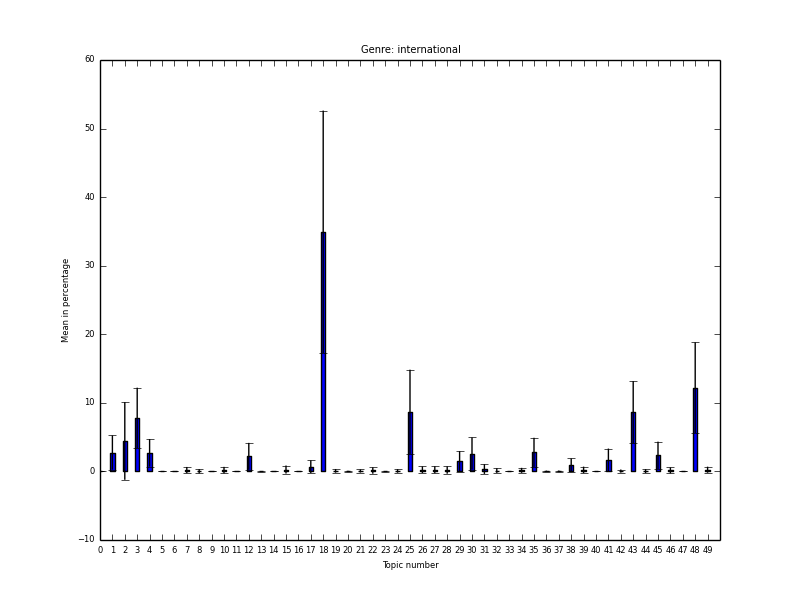
\includegraphics[width=\textwidth]{bar_charts/international.png}
                \caption{Genre International}
                \label{fig:topicdist_international}
        \end{subfigure}
        \caption{Topic distibution for different genres}\label{fig:topicdist}
\end{figure}

\begin{figure}
\begin{mdframed}
cause leader sun nigga bastard push verse \\
end account high mountain ballin trash yall \\
pen tears writing instrumental gucci like chorus \\
rule best clean legit line curtains way heroin \\
proven nothin yo find 1 aint oh \\
ride every rising gambino
 \end{mdframed}
\caption{Song of length $40$ generated in genre \textit{rap} with $\alpha=\beta=0.7$, 20 topics and 30 iterations of Gibbs sampling}
\label{text:rap_song}
\end{figure}